\section{Geometrie}
\subsection{Planimetrie}
\subsubsection{Strahlensätze}
\subsubsection{Satz des Pythagoras}

\subsection{Pythagoras}


%\begin{figure}[htb]
%\begin{center}
%	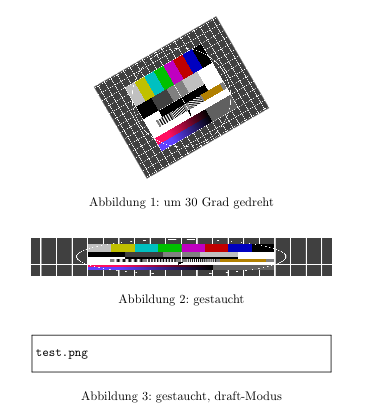
\includegraphics[height=1in,width=1in,angle=-90]{sections/08_Geometrie/pythagoras.standalone.pdf}
%\caption{This is a figure.}
%\end{center}
%\end{figure}



\subsubsection{Höhensatz des Euklid}
\subsubsection{Kathetensatz}

\subsubsection{Kreis}


\begin{figure}
    %\centering
    \subfloat{
	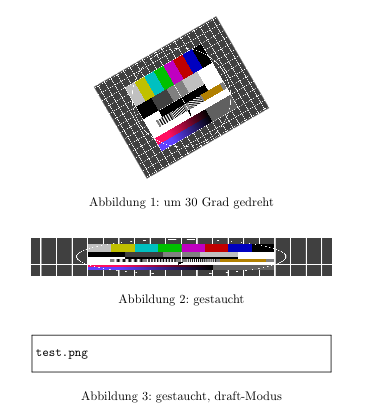
\includegraphics[height=2in,width=2in,angle=-90]{sections/08_Geometrie/pythagoras.standalone.pdf} 
    }\hfill
    \subfloat{
      \begin{minipage}[t]{120mm}
   	$A = \frac{d^2 \cdot \pi}{4}$ \\
	$U = d \cdot \pi  $
      \end{minipage}
}
  % \caption{Abbildungsname}
  % \label{fig:decision-tree}
\end{figure}

\subsection{Stereometrie}
\subsection{Trigonometrie}
\subsection{Geniometrie}